\section{Implementers' guide}\label{sec:implguide}
% \sideboxbegin{o}
% This section presents the limitation encountered while integrating the functionalities of Trace\textit{a} into SysMLv2.
% \sideboxend



\subsection{Example usage scenario}
\begin{figure}[h]     
	\centering
	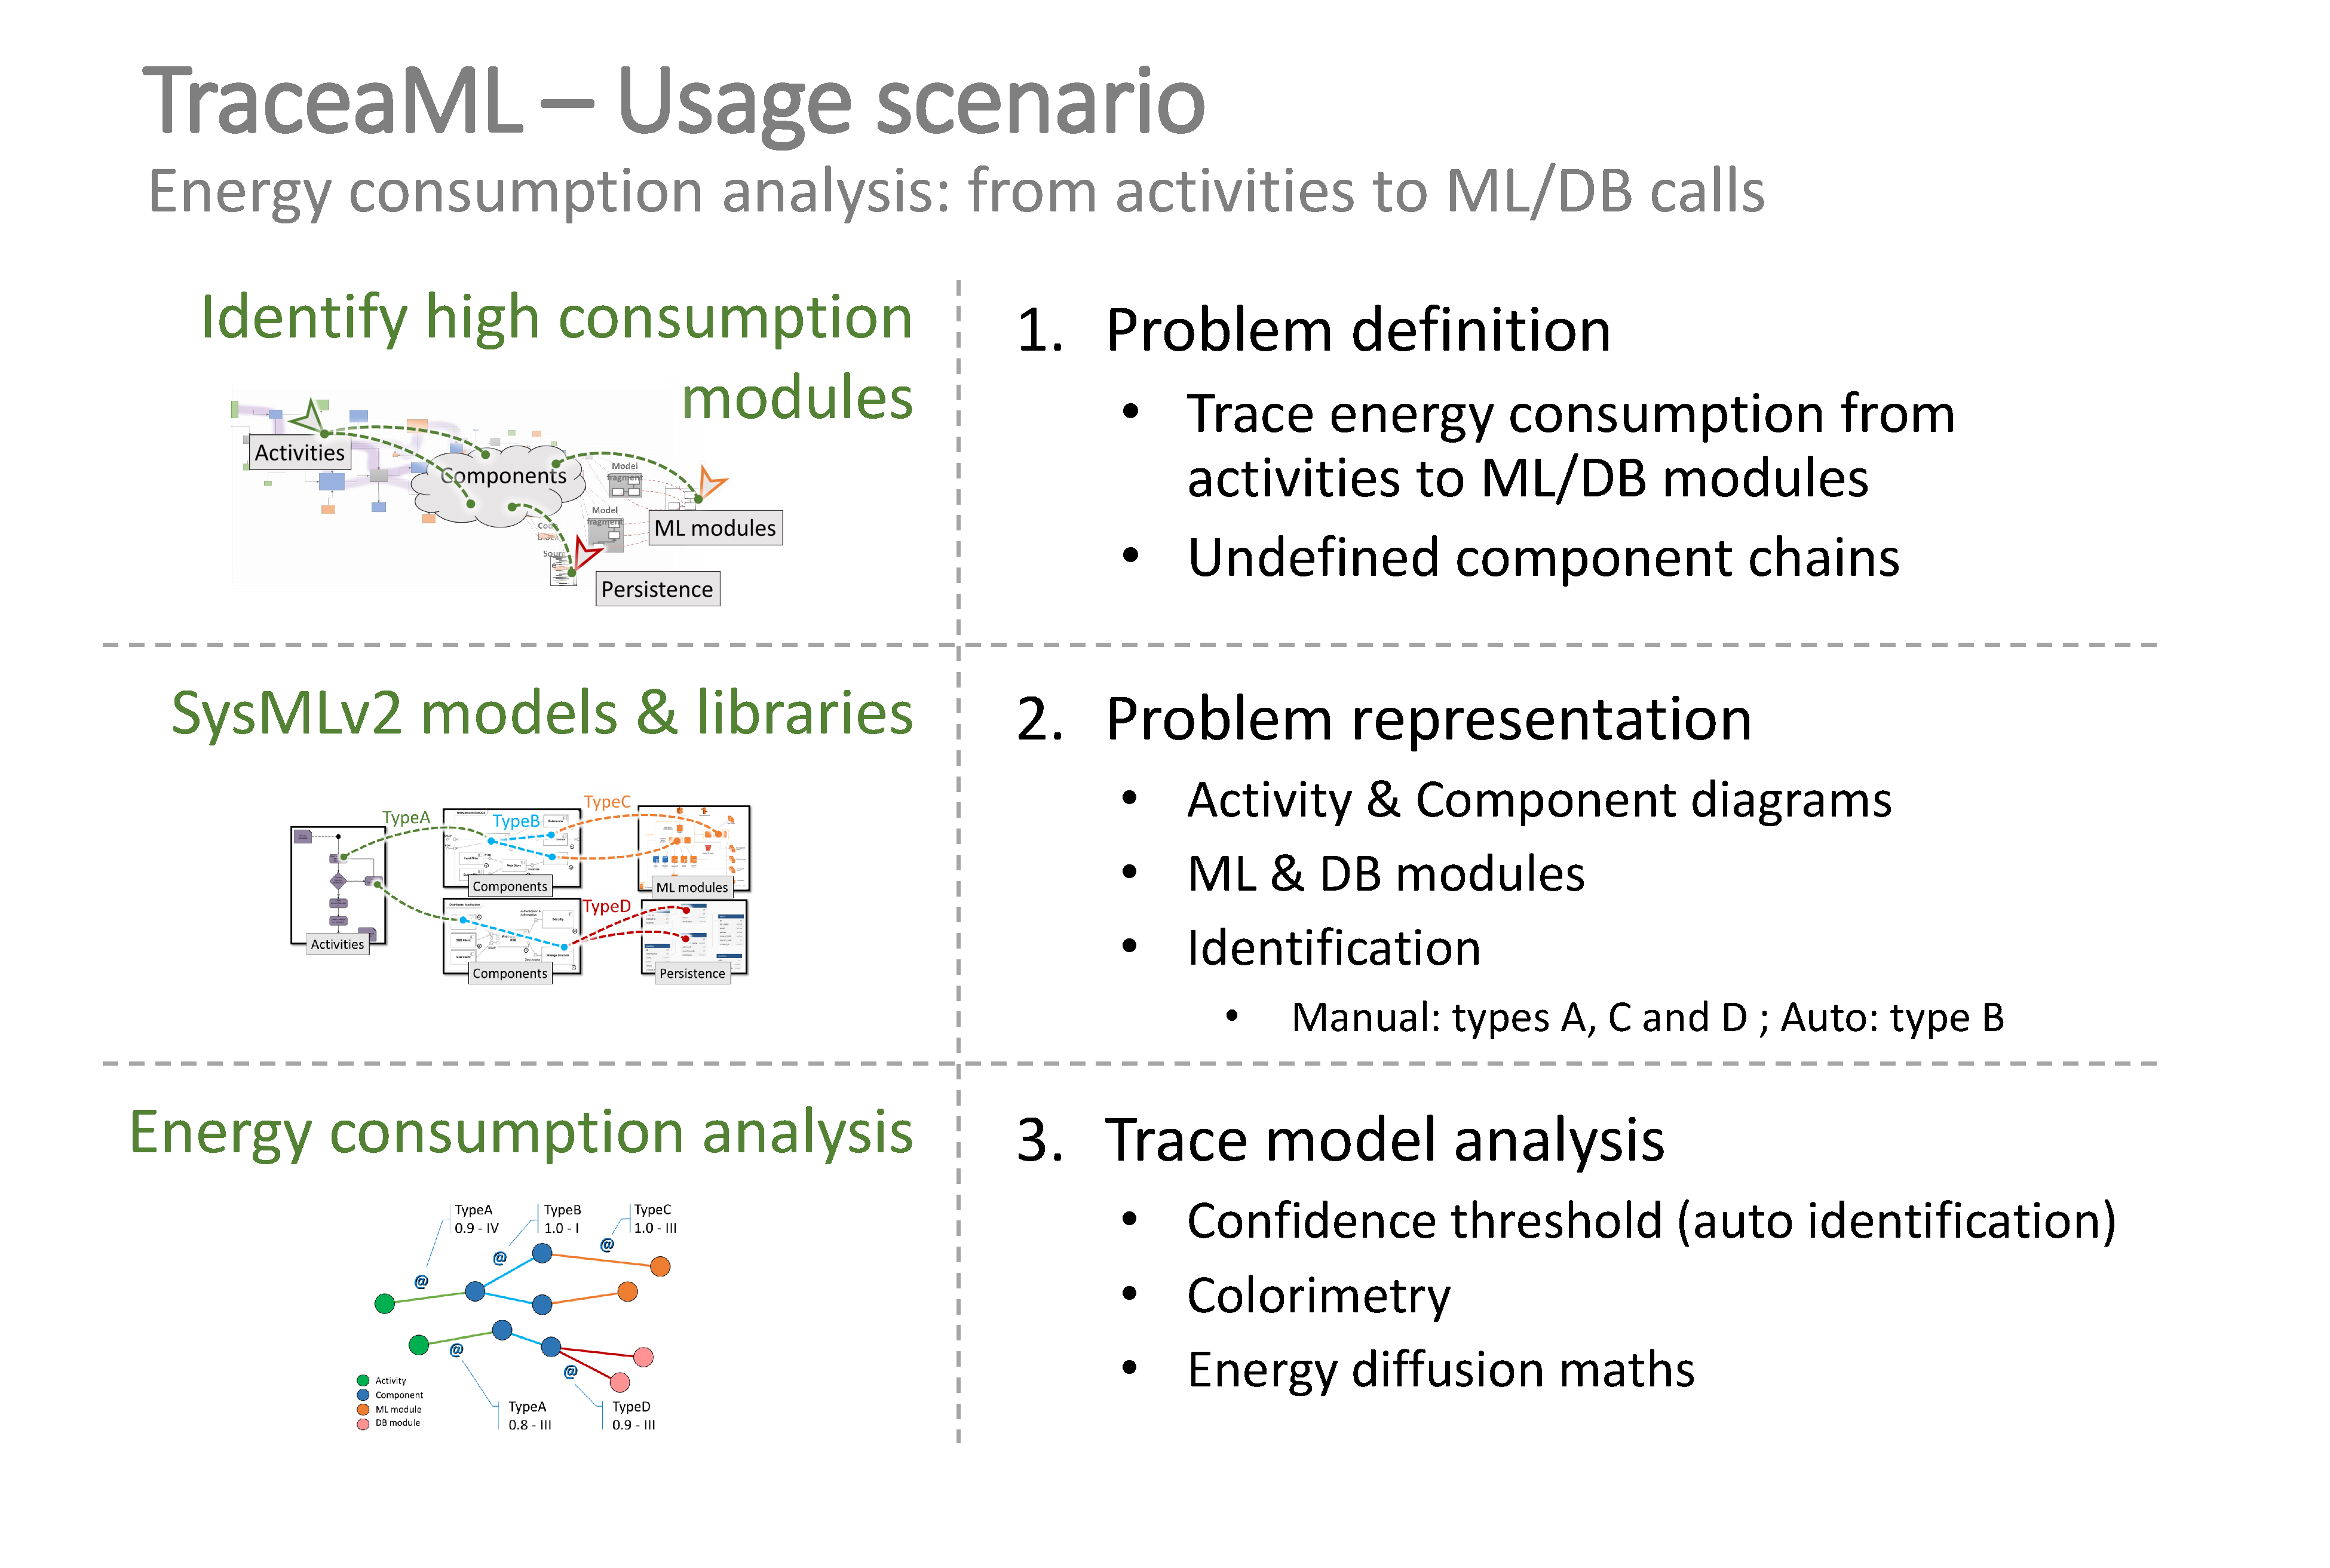
\includegraphics[width=.99\linewidth]{images/scenarionrj.pdf}
	\caption{Use case: Energy consumption analysis.}
	\label{fig:scenarionrj}
\end{figure}


\subsection{Problem definition}
\begin{figure}[h]
	\centering
	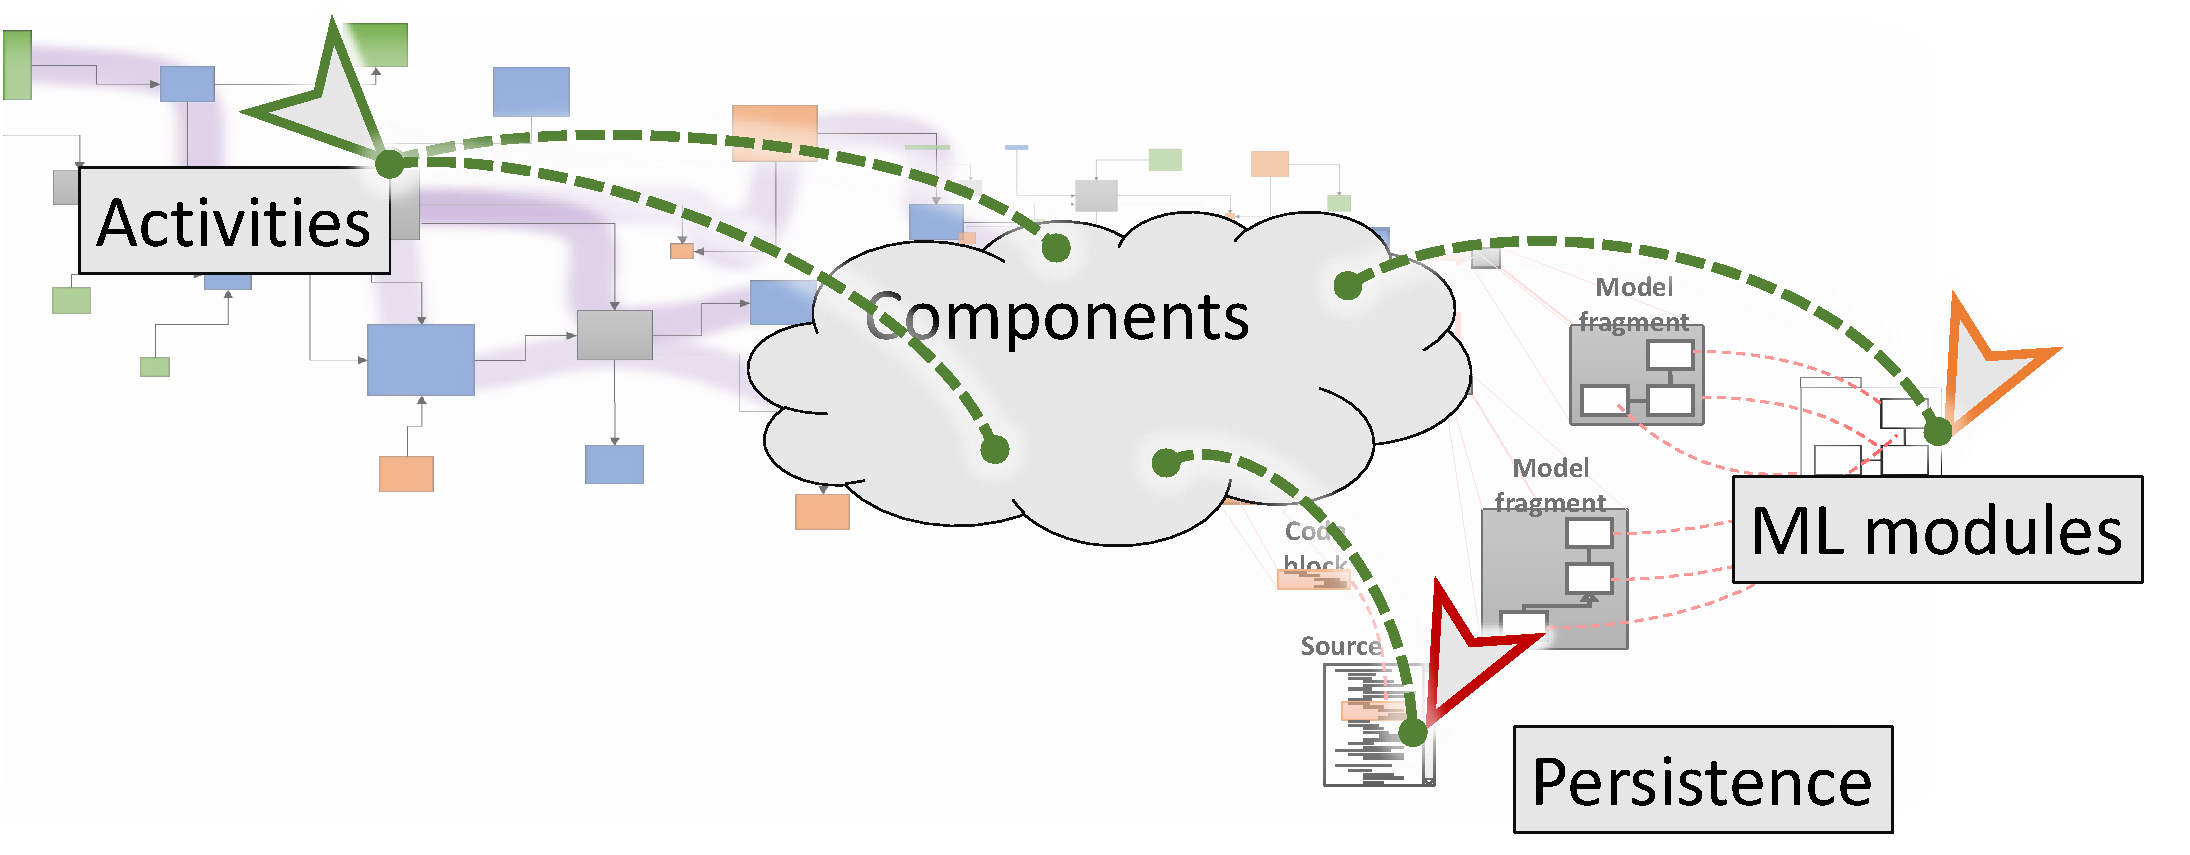
\includegraphics[width=.6\linewidth]{images/energy1.pdf}
	\caption{Problem statement.}
	\label{fig:energy1}
\end{figure}

\subsection{Problem representation}
\begin{figure}[h]     
	\centering
	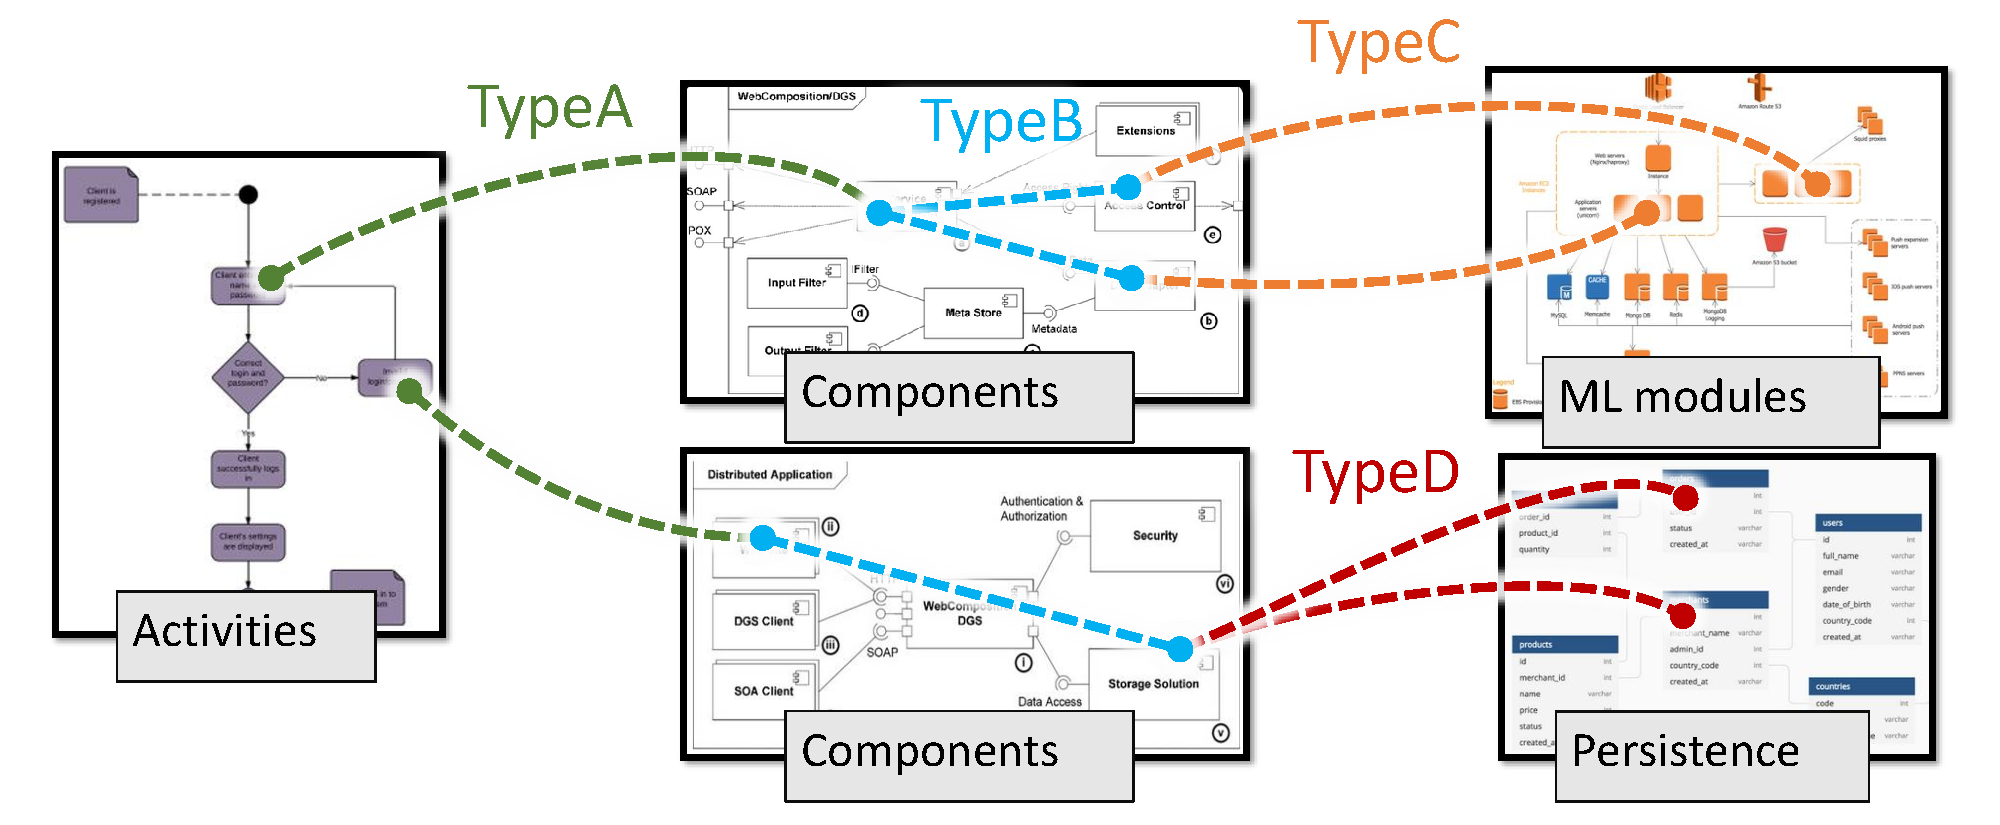
\includegraphics[width=.8\linewidth]{images/energy2.pdf} 
	\caption{Problem representation.}
	\label{fig:energy2}
\end{figure}

\subsection{Trace model analysis}
\begin{figure}[h]     
	\centering
	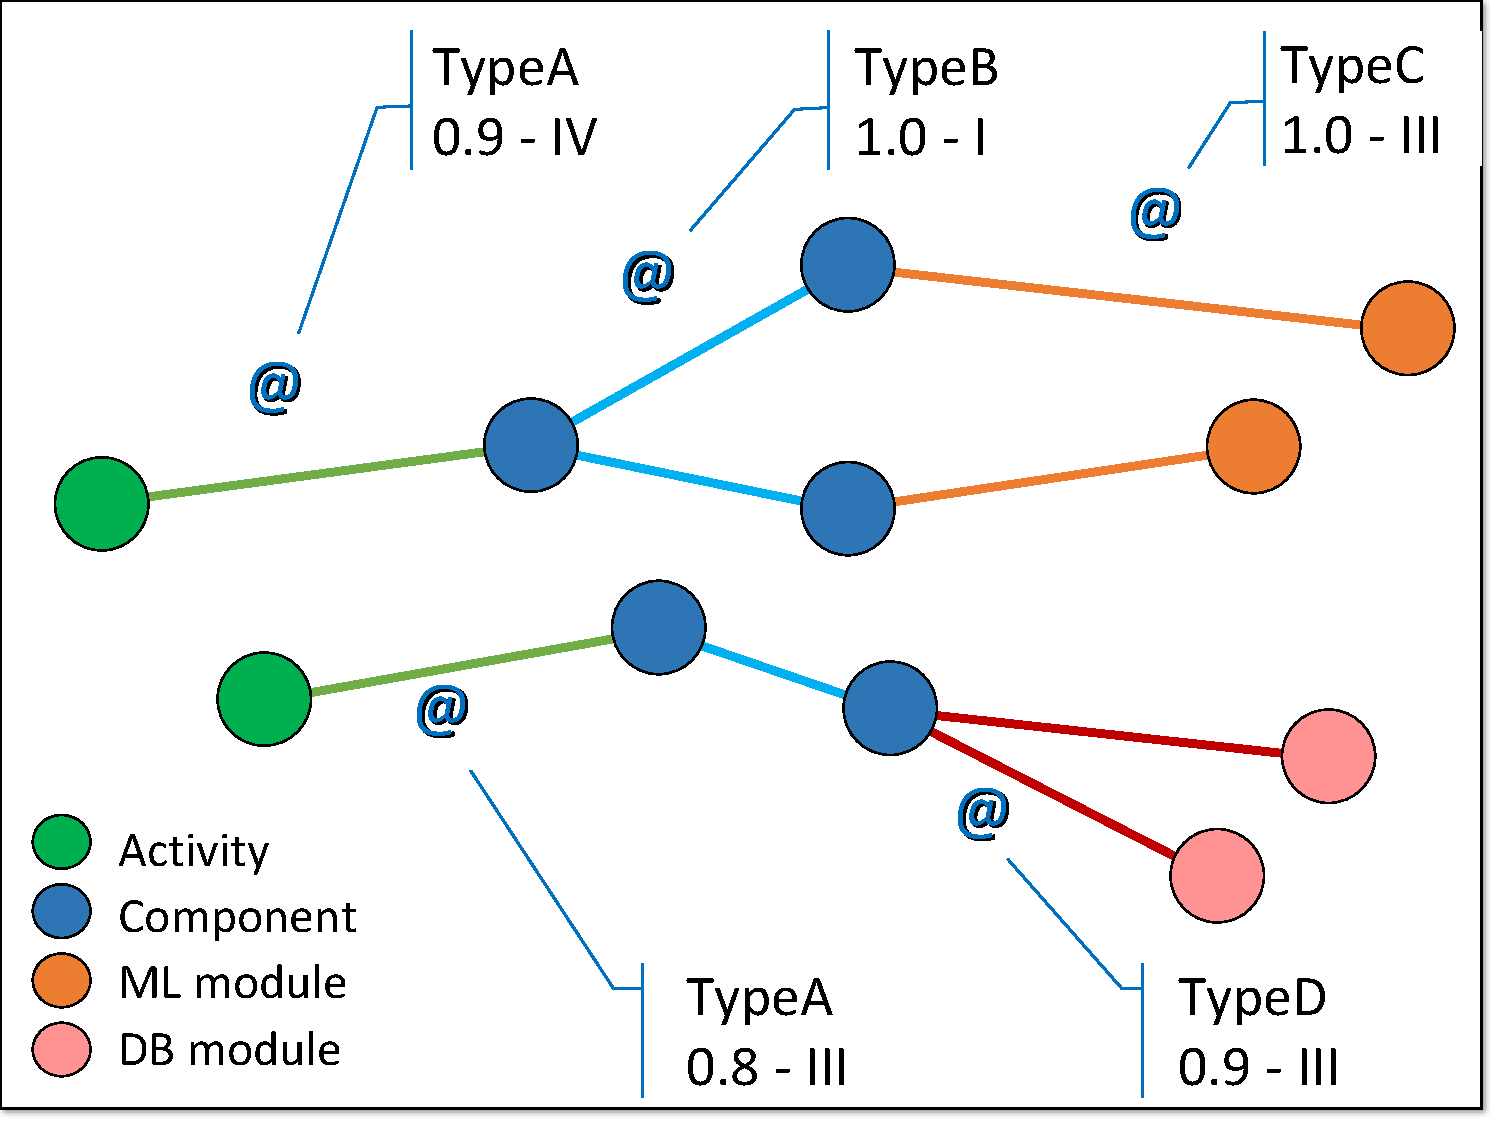
\includegraphics[width=.5\linewidth]{images/energy3.pdf}
	\caption{Trace model representation.}
	\label{fig:energy3}
\end{figure}

\subsection{Toward multi-criteria apprehension}

